\chapter[Synthesis]{Synthesis}
\label{cha:Chapter6}
\newpage

This thesis aims to contribute towards efforts in large-scale land cover mapping, with an emphasis on the benefits of combining several datasets from different sources and of different types. It presents different steps of a methodology to extract training data from multiple rich human-annotated datasets and overlay them on Earth observation data from diverse sources, and details the challenges and benefits of doing so while creating land cover maps that navigate the trade-off between spatial, temporal, and thematic resolution, as well as quantity and allocation accuracy.

This thesis, especially in its first two chapters, summarises a relatively 'applied' line of research. Besides the chapters themselves, several datasets were produced, and have been published as open data (CC-BY):
\begin{enumerate}
    \item 2000-2020 quarterly Landsat composites at 30m resolution and 7 bands;
    \item 2016-2019 quarterly/annual Sentinel-2 composites at 10-30m resolution, depending on the band;
    \item An Ensemble Digital Terrain Model of Europe at 30m resolution;
    \item 2000-2019 annual Land Use / Land Cover maps of Europe at 30m resolution and 43 classes;
    \item Five annual land cover maps of five European countries (Belgium, Czechia, Germany, Luxembourg and The Netherlands) at 30m resolution and 8 classes, whose class proportions match Eurostat area estimates.
\end{enumerate}
The third chapter of the thesis describes relatively more innovative attempts to model land cover in a way that is faithful to area estimates. The proposed algorithm (IMP) may have further uses and implications; these will also be discussed in this synthesis chapter. It is divided into two sections: the first summarizes contributions to the research objectives formulated in Section~\ref{sec:research_objectives}; the second reflects on these contributions, offering perspectives on future research opportunities. 

\section{Main Findings}
    The chapters of this thesis each address multiple research questions and should be considered jointly in this synthesis. Their results will be discussed from the perspective of the research questions; each question is discussed below.
    
    \subsection{What are the benefits and challenges of combining multiple large time-series and static EO datasets into Analysis-Ready Data for the purpose of land cover classification?}
    \label{syn:rq1}

        This research question was largely explored in chapters 2 and 3. Chapter\@~\ref{cha:chapter2} details the construction of an Earth observation data cube from several sources (Landsat, Sentinel-2 and several DTMs), and includes experiments that investigate the performance of land cover models using different combinations of these datasets. Chapter\@~\ref{cha:chapter3} uses most of this data cube to train a single LULC classification model, which is subsequently used to create annual maps of Europe between 2000 and 2019. 

        \subsubsection{Benefits}
    
            Our land cover experiments in Chapter\@~\ref{cha:chapter2} show that random forest models trained on the largest combination of datasets achieved the highest classification accuracy during cross-validation and that models trained on Landsat and DTM data achieved the highest accuracy on test data. This is in line with other work reporting that including auxiliary variables in the feature space can improve performance \citep{zhu2016optimizing, hurskainen2019auxiliary, hosseiny2022urban, santos2012multiscale}.

            Chapter\@~\ref{cha:chapter2} also details the creation of an Ensemble DTM which was more accurate than its four source datasets, with a RMSE 6.544 vs RMSE of 8.451-9.900. This proves that in the case of continuous variables, different versions or representations of that variable can be used as input for a machine learning algorithm, and that the predictions by this algorithm can be more accurate.
            
            In Chapter\@~\ref{cha:chapter3}, the top 15 most important variables of the ensemble land cover model contain data from six sources: Several bands from two satellite programs (Landsat and MODIS), long-term probability of surface water occurrence \citep{pekel2016high}, geometric temperature \citep{kilibarda2014spatio}, multiple DTM variables, and the cost distance to the nearest coastline (see Figure~\ref{fig:variable_importance}). 
    
        \subsubsection{Challenges}
            
            Experiments in Chapter\@~\ref{cha:chapter2} showed that models using the full feature space (Landsat, Sentinel-2 and DTM) achieved the highest classification accuracy, with different datasets improving the results for different land cover classes. This is supported by variable importance in Chapter \ref{cha:chapter3}: Data from four different sources (Landsat, surface water frequency, DTM, and distance to coast) were among the top 15 of 200 variables for LULC modeling.
            
            While it is clear that combining different datasets into one feature space can improve model performance, there are some challenges:
    
            \textbf{Spatial resolution}: Overlaying different raster datasets onto training samples may yield high accuracy (like in Chapter\@~\ref{cha:chapter2}), but can cause artifacts in the shape of low-resolution raster cells creating maps at the highest resolution among the used datasets. Fortunately, recent findings suggest that certain modeling techniques such as convolutional neural networks can counteract this effect \citep{robinson2019large}. Chapters\@~\ref{cha:chapter3}\@~and\@~\ref{cha:chapter4}, we used low-resolution MODIS data used as part of the feature space. To avoid artifacts, we smoothed it while resampling it to a 30~m resolution, but this is a very unsophisticated way and may have lead to the loss of a lot of explanatory power. This is also reflected by its low position in the variable importance of the ensemble model in Chapter\@~\ref{cha:chapter3}.

            \textbf{Temporal resolution} can be subdivided into the temporal resolution of the feature space and of the mapped units. It is essential to have a high temporal resolution in the feature space to correctly detect and distinguish different vegetation types due to the temporal dynamics of their phenology. 
            
            The time range represented by a single map has different implications for the accuracy of different classes. In Chapters\@~\ref{cha:chapter3}\@~and\@~\ref{cha:chapter4}, we chose to make annual maps, and in Chapter\@~\ref{cha:chapter3}, we made annual maps for each consecutive year. This does not work equally well for each class. For example, mapping classes that only periodically cover a certain patch of ground, such as crops, or areas that are prone to different water levels, such as flood plains. At a high thematic resolution, this problem may be minimal: a change of crops due to crop rotation will still be cropland, but when mapping different crops, this will quickly become problematic. Another example from Chapter\@~\ref{cha:chapter3} is \textit{Burnt areas}, which was among the least accurately mapped classes. This is likely due to the fact that these areas don't stay \textit{Burnt} for a long time.

            \textbf{Class balance}: Collecting land cover observations from multiple sources requires consideration of the quality and type of each component dataset. We sampled points from polygons from different datasets, which all have their own problems. For instance, CORINE's large minimal mapping unit can lead to sampled points of an urban area falling within a garden, and therefore being a bad example of a 'buildings' class. Similarly, some classes with small or narrow patches (e.g. roads) can be underrepresented in such datasets, which leads to underrepresentation in the resulting training set. In volunteered geographical information, errors can come from different sources. For example, when collecting \textit{Greenhouse} data for chapter 5, we encountered greenhouses labeled in many different terms, languages, and spelling errors (\textit{'greenhouse', 'greenhouse\_horticult', 'glasshouse', 'greenhouses', 'greehnouse', 'greenhosue', 'greenhuose'}).

            In Chapter\@~\ref{cha:chapter3}, we did not pay any attention to this issue and selected one point per polygon, which lead to some classes being drastically underrepresented and more inaccurately classified than expected, even with a large legend of heterogeneous combinations of land use and land cover classes such as CORINE. In chapters 2 and 4, we only used the LUCAS points because the emphasis was on the benefits of combining EO data sources and the effects of the IMP algorith, respectively. In chapter, 5, however, we tried to improve the training data extraction method by making the number of sampled points dependent on the size of the polygon.

            \textbf{In general}, the more data you combine, the more chance there is that an incompatibility or inconsistency creeps in and causes artifacts or inaccuracies later in the line. Careful planning and proper testing can ameliorate this, but with increasing data complexity, it becomes exponentially more difficult.
            

    \subsection{To what extent does training data from multiple times and places improve the accuracy and generalization of land cover classification?}
    \label{syn:rq2}
    
        The land cover experiments in chapters 2 and 3 investigate the generalization potential of models trained on data from a single year, and those trained on data from several years. Results from both chapters show that models trained on samples from different years were more accurate; both on years with available training data, and on unseen years.

        In the land cover classification experiments of chapter~\ref{cha:chapter2}, the model that was trained on a small multi-year landsat-only outperformed the model trained on landsat, sentinel, and DTM data on the test set. This suggests there is a unique benefit in training a model on data from a larger time range.
        
        In chapter~\ref{cha:chapter3}, we combined LUCAS points with samples extracted from CORINE polygons to create a training dataset with samples from 8 years (see table~\ref{tab:cv_annual}). Cross-validation showed that the weighted F1-score of the model was more consistent through time than through space (with standard deviations of 0.135 per year and 0.150 per 30~km tile, respectively). 
        In particular, our map of 2017 was validated on the points collected by \citep{jenerowicz2021validation} to validate the S2GLC maps made by \citet{malinowski2020automated}, and achieved a similar accuracy without having training data from 2017 and operating on a lower spatial resolution.

        \subsubsection{Dealing with bias}
        Combining training data from several locations and times can introduce bias in the model because the proportion of classes might not match the proportions on the ground in the mapped area in a given time frame. Our results in Chapter\@~\ref{cha:chapter2} show that the ensemble model was much less accurate in Southern Europe than in Central and Northern Europe. We found a weak but significant positive correlation between the number of training samples and the F1-score in 30~km tiles across Europe (see Figs.\@~\ref{fig:cv_spatial}\@~and\@~\ref{fig:tiles_support_vs_v1}. We did not analyze whether this was due to low precision or recall, but it is likely that differences in proportions of locally abundant such as \textit{Sclerophyllous vegetation}, which are mostly found around the Mediterranean, played a role in lowering the accuracy where they occur more than the European average. On a large scale, the spatial distribution of its probabilities matches its geographical spread quite well (See Fig.\@~\ref{fig:sclerophyllous}) but this class was hardly predicted in the hard-class map, being frequently overshadowed by \textit{coniferous forest} and other vegetation types.  

        \begin{figure}[H]
            \centering
            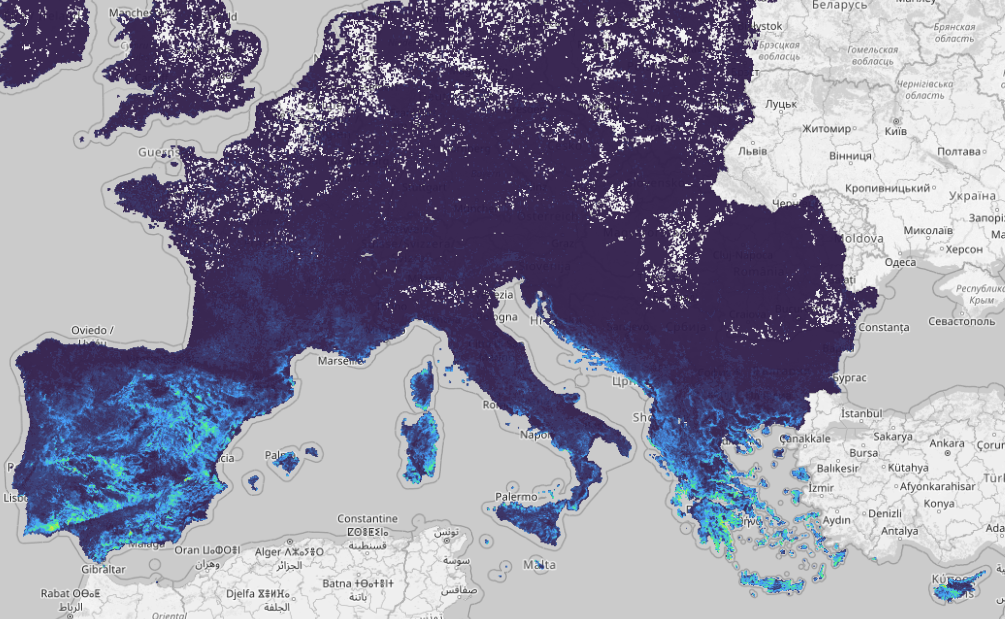
\includegraphics[width=1\linewidth]{figs_06/sclerophyllous.png}
            \caption{Predicted probabilities for sclerophyllous vegetation}
            \label{fig:sclerophyllous}
        \end{figure}
        
        The proportional mapping approach demonstrated in Chapter\@~\ref{cha:chapter4} may provide a solution to this issue. In that chapter, we mapped the 8 level 1 LUCAS land cover classes across five years and five countries, and compared the performance of models trained only on the country they mapped with the performance of a model that was trained on data from multiple European countries. We found that proportional maps based on predictions by the general model were of similar accuracy to both the maximum probability assigned and proportional maps based on probabilities predicted by the less biased local models. This suggests it is possible to train one model that can recognize many classes. If such a model is well-calibrated within each class and the top 5\% of predicted probabilities for e.g. \textit{sclerophyllous vegetation} are indeed the most likely to actually be that class, even if they are overshadowed by more common classes, local area estimates can be used to force them to the forefront in areas where such classes are known to be more numerous. 
        

    \subsection{How does the number and type of classes in a legend affect the accuracy of land cover classification?}
    \label{syn:rq3}

        In Chapter\@~\ref{cha:chapter3}, we found large differences in hard-class accuracy between the three different levels of the CORINE legend: At level 3, only 11 out of 43 classes were mapped with an F1-score above 0.5 (Discontinuous urban fabric, industrial or commercial units, non-irrigated arable land, rice fields, broad-leaved forest, coniferous forest, bare rocks, glaciers and perpetual snow, peat bogs, and water bodies. At level 2, this was 9 out of 14 classes, and at level 1, all 5 classes. At level 3, we can see a positive relationship between the number of samples ('support' in table \ref{tab:cv_accuracy_lvl3}) and the F1-score, although there are classes with many samples that still scored poorly. There is a number of error sources: 

        Firstly, some of these classes are 'mixed types' such as \textit{Complex cultivation patterns}, \textit{Agriculture with significant natural vegetation} and \textit{Mixed forest}. Some other classes occur mostly at a sub-pixel level, in effect being mixed classes with whatever class they border. For instance, \textit{roads and rail networks and associated land} in Chapter\@~\ref{cha:chapter3}. Stretches of road or rail infrastructure that are wider than 30~m are relatively rare, and this type of land cover is often very close to other classes such as buildings. If there are classes in the same (level of the) legend, these classes 'compete', even if a prediction for any of them would be true. 
        Second, some LULC classes have the same land cover, but differ in land \textbf{use}, such as \textit{Pasture}, \textit{Natural grasslands}, and \textit{Airports} (which also have significant grasslands, see Figure \ref{fig:airport_grass}). Properly distinguishing those classes may require higher temporal and spectral resolution or feature engineering to detect differences in mowing policy or grass species. 
        
        These mixed class and land use errors largely disappeared when aggregating classes to a level in the hierarchy where mixed nature or land use distinctions ceased to matter, such as \textit{313: Mixed Forests} to \textit{CLC 31: Forests and seminatural areas}. This only works for classes that are placed in a logical order in the legend: For instance, \textit{Pastures} and \textit{Natural grasslands} are considered as completely different LULC types even at the highest level of the legend, where they are aggregated to \textit{Agricultural areas} and \textit{Forest and semi-natural areas}, respectively. In the S2GLC legend, however, we both aggregated these grass classes to \textit{Herbaceous Vegetation}, which was much more effective. This applied to the S2GLC legend in general: When we summed the probabilities of all classes according to the S2GLC scheme, we achieved similar or higher accuracy than the S2GLC land cover maps. This means that training a model on many classes, even more classes than 'needed' for a specific use case, does not intrinsically harm its accuracy in a simpler legend, even when the land cover predictions are inaccurate at the highest level of detail.
    
        \begin{figure}[H]
        \centering
        \begin{subfigure}[b]{0.48\textwidth}
            \centering
            \caption{OpenStreetMap}
            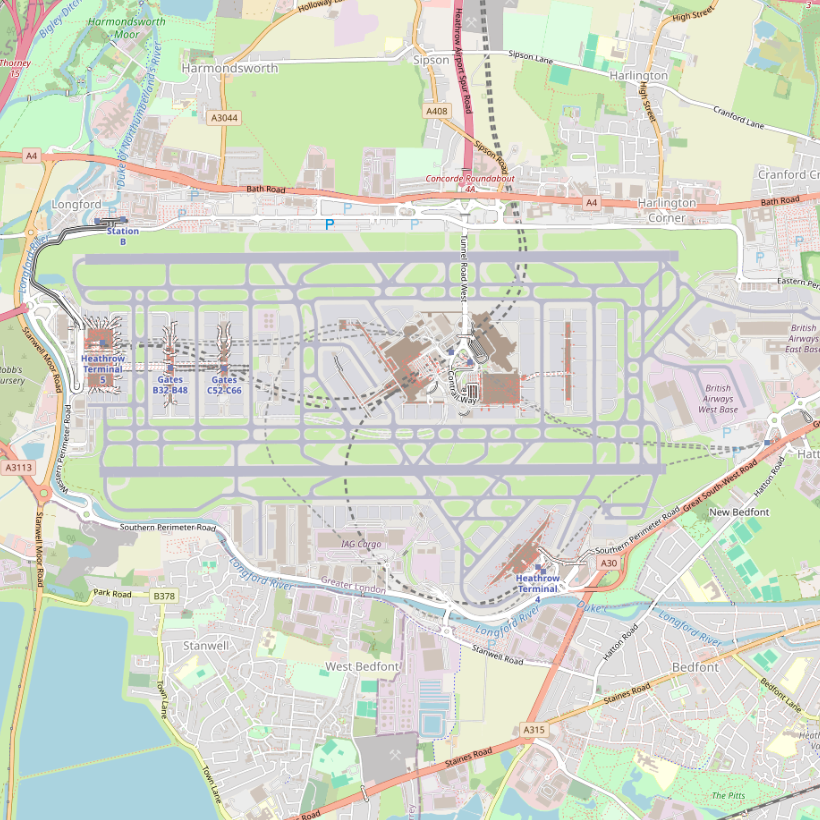
\includegraphics[width=\textwidth,height=0.7\textwidth]{figs_06/heathrow_osm.png}
            \label{fig:heathrow_osm}
        \end{subfigure}
        \hfill
        \begin{subfigure}[b]{0.48\textwidth}
            \centering
            \caption{CORINE Land Cover}
            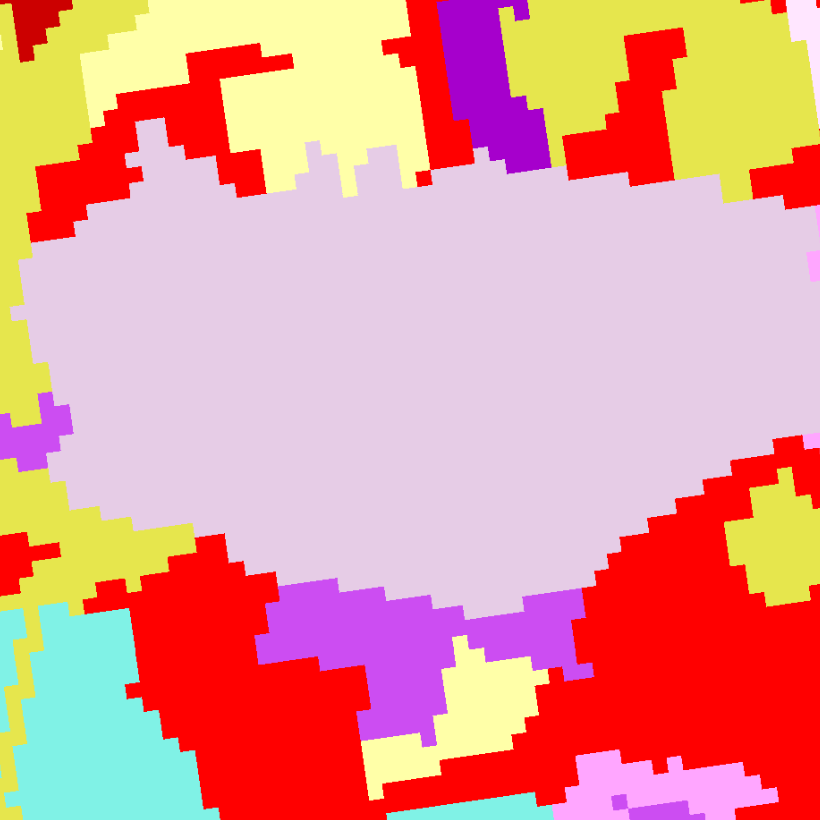
\includegraphics[width=\textwidth,height=0.7\textwidth]{figs_06/heathrow_clc.png}
            \label{fig:heathrow_corine}
        \end{subfigure}
        
        \vspace{0.5em}
        
        \begin{subfigure}[b]{0.48\textwidth}
            \centering
            \caption{Probability for \textit{Airports}}
            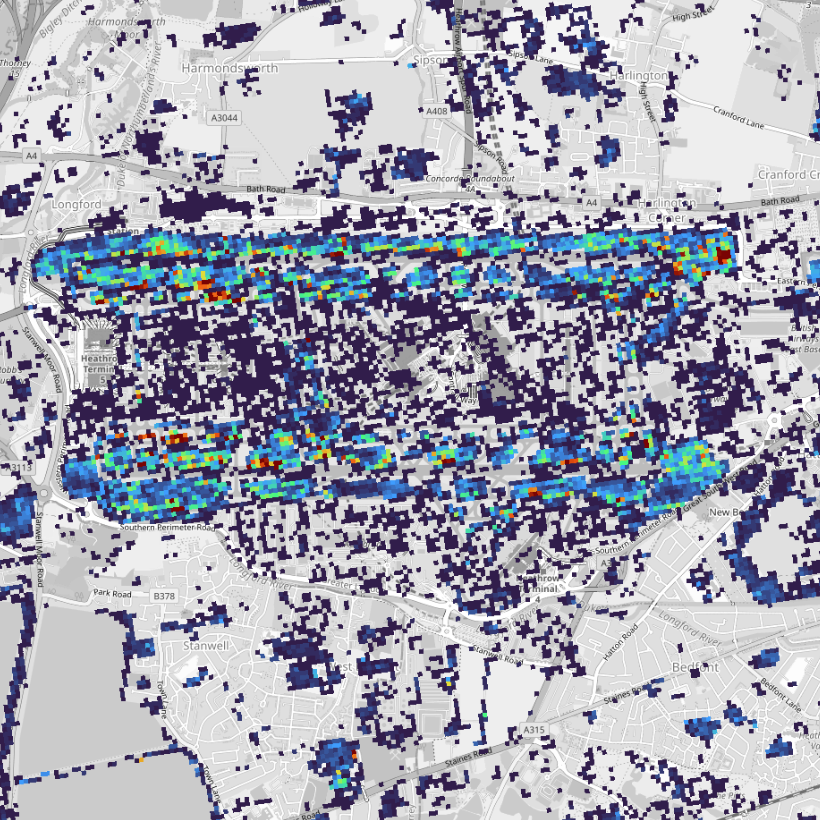
\includegraphics[width=\textwidth,height=0.7\textwidth]{figs_06/heathrow_p_airport.png}
            \label{fig:heathrow_airport}
        \end{subfigure}
        \hfill
        \begin{subfigure}[b]{0.48\textwidth}
            \centering
            \caption{Probability for \textit{Industrial and commercial units}}
            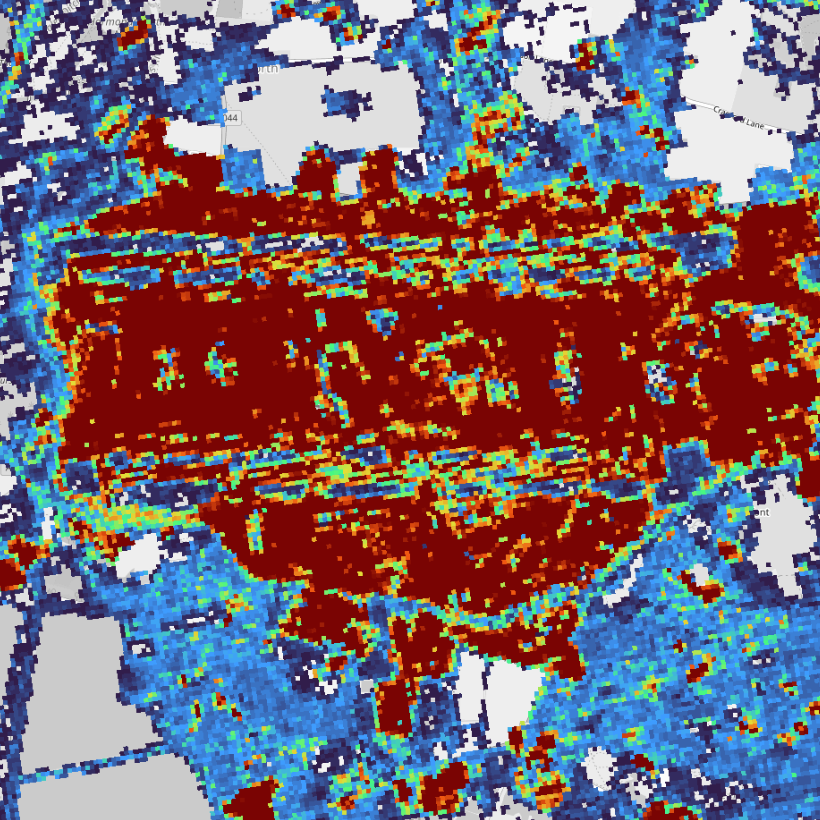
\includegraphics[width=\textwidth,height=0.7\textwidth]{figs_06/heathrow_p_industrial_commercial.png}
            \label{fig:heathrow_industrial-commercial}
        \end{subfigure}

        \vspace{0.5em}
        
        \begin{subfigure}[b]{0.48\textwidth}
            \centering
            \caption{Probability for \textit{Pastures}}
            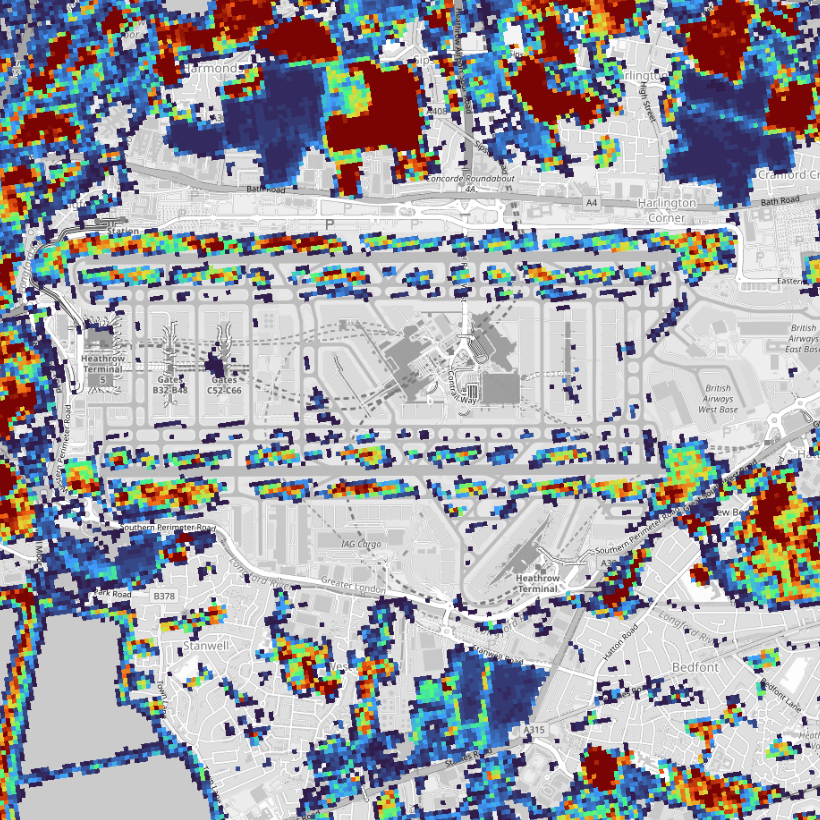
\includegraphics[width=\textwidth,height=0.7\textwidth]{figs_06/heathrow_p_pastures.png}
            \label{fig:heathrow_industrial-commercial}
        \end{subfigure}
        \hfill
        \begin{subfigure}[b]{0.48\textwidth}
            \centering
            \caption{Hard-class classification}
            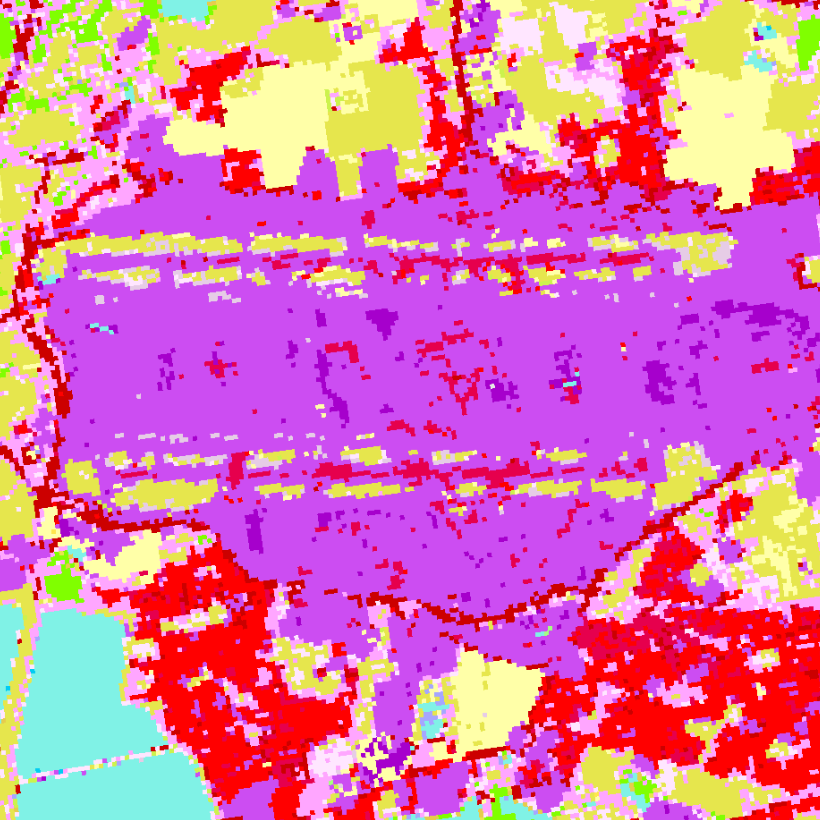
\includegraphics[width=\textwidth,height=0.7\textwidth]{figs_06/heathrow_lulc.png}
            \label{fig:heathrow_industrial-commercial}
        \end{subfigure}
        \label{fig:airport_grass}
        \caption{Comparison of CORINE Land Cover and LULC classification from Chapter\@~\ref{cha:chapter3} for Heathrow Airport, London, in 2018. Note that the LULC classification did a decent job classifying the non-residential buildings cultivated grassland that together make up the airport, but failed to assign them to the actual \textit{Airport} class.}
        
        \end{figure}

            
    \subsection{What is the effect of enforcing correct class proportions on map accuracy?}
    \label{syn:rq4}
 
        In Chapter\@~\ref{cha:chapter4}, we created annual maps of 5 European countries. For each country, we predicted probabilities with a local model that was trained only on data from that country. We also predicted probabilities for each country with a model that was trained on a larger, pan-European dataset. We then made hard-class maps of each country and year in two ways: By maximum probability assignment, and with a novel algorithm: Iterative Mapping of Probabilities (IMP).
        
        The IMP algorithm was developed as a tool to produce maps that match existing area estimates without sacrificing accuracy. Our experiments in Chapter\@~\ref{cha:chapter4} show that classifications by IMP tend to be \textit{more accurate} than those by maximum probability assignment, especially in the case of models that are biased to over- and underpredict certain classes. 
        
        Results showed that maximum probability maps using the probability of the local models tended to be more accurate than those by the general model, but this was not the case when using IMP instead of maximum probability assignment. The maps created by IMP were however of equal or better accuracy than those made with maximum probability assignment, while having class proportions as estimated by Eurostat. The effect of IMP on accuracy  can be summarized as sacrificing precision (user accuracy) of some classes, to raise recall (producer's accuracy), with a net benefit to higher weighted F1-scores.

        \subsubsection{Future research}
        
        Essentially, IMP quantifies the bias of a model when compared to a given class proportion estimate and uses the iteration probability thresholds to impose its own bias on the model predictions, minimizing the difference between precision and recall.
        While class-wise precision and recall values of proportional maps were closer to each other than those of maximum probability maps, they were not identical. While Eurostat area estimates are considered to be quite reliable, a direct class count from a dataset is by definition 100\% accurate. It is likely that using these counts could use to further harmonize precision and recall on a class-by-class basis. If this is true, IMP can potentially be used to quantify either how representative a validation dataset is for its study area, or the accuracy of a class proportion (area) estimate. Additional experiments that did not make it into the thesis provide strong suggestions that this is true, and we will keep researching this in the near future.
        
        Chapter\@~\ref{cha:chapter4} showed that IMP provided a greater accuracy improvement to models that were trained on data with a different class distribution than the area they mapped. This means that IMP can be used to optimize the predictions of large land cover models to a regional context without requiring new training or predictions. It also means that IMP can learn the bias of a model if the model is validated in an area for which class proportions can be estimated; the quantification of this bias can then be stored, and used to make proportional maps of areas for which class proportions are not available. This too is a promising line of research that will be continued after this thesis. 

        If reliable, trusted validation data exists for an area, IMP can be used to compare the accuracy of different area estimates by making hard-class maps for each area estimate. The area estimate that matches the reality on the ground most closely should allow IMP to produce the most accurate map. When used this way, IMP could be used to settle disputes about quantities of land cover and land cover change.

        \subsubsection{Wider applicability}
        
        The ability of IMP to quantify and correct model bias extends its usage beyond land cover classification. It can be used for any type of machine learning task where class proportions can be either estimated, targeted, or dictated, and where bias must be quantified. Any field that utilizes machine learning models and faces challenges with class imbalance, representation bias, or requires models to perform accurately across diverse and potentially underrepresented groups could use the algorithm to enhance model fairness, accuracy, and generalization.
        
        For example, in predictive policing and recidivism prediction, biases in the training data can perpetuate and amplify societal biases. Reducing the bias in such models could contribute to fairer decision-making in the criminal justice system \citep{berk2021fairness, dressel2018accuracy}. Financial institutions often use machine learning models for credit scoring and risk assessment. The training data can be biased due to historical decisions and social demographics, potentially leading to unfair assessments. A post-hoc correction algorithm could mitigate these biases, leading to fairer credit scoring and risk assessment models \citep{chen2018why, kamiran2012data}. 

\section{Reflection and outlook}

    This thesis presents a transparent, reproducible framework for combining data from various sources to create detailed, consistent maps. Its chapters show examples of how to combine earth observation and land cover data from multiple sources, pre-process and harmonize them, and make annual maps with many classes. It shows how to deal with the problems
    
    Combining several datasets from different times and regions to create large and rich training datasets is a challenging task. It requires knowledge of available data sources, technical skills, and extensive spatial, temporal, and thematic harmonization work. This thesis shows that such a dataset can be used to train a model that classifies many classes. While the accuracy at full thematic depth is lacking compared to those of other recent products, we present proof that the hierarchical nature of complex legends can be leveraged to reach accuracy that is on par with the state of the art. We also show that there are  benefits to training a model on data from different times, even without performing any kind of time-series analysis. Finally, we show that it is possible to incorporate class proportions such as area estimates into the workflow to create land cover maps that not only match these proportions, but are more accurate than maximum probability maps.

    We have published the code and data that we used and produced in this thesis in the hope that it is useful to other modelers, especially those who are not experts in remote sensing. The analysis-ready feature space and harmonized training datasets can be used by anyone to improve our method and maps. The predicted probabilities of Chapter\@~\ref{cha:chapter3} can be used as input for ensembles to map other types of land cover, potentially much more accurate than the probabilities themselves, just like has been suggested by the creators of DynamicWorld \citep{brown2022dynamic}.

    This thesis not only contributes to the field of remote sensing by enhancing methods for land cover mapping but also sheds light on the role of data integration and methodological innovation in addressing current limitations. Nonetheless, the journey toward comprehensive, dynamic, detailed representation of the Earth's surface is far from complete. As we stand on the threshold of new discoveries and technological frontiers, we are propelled to ask a fundamental question: What is necessary to \textit{map everything, everywhere, all the time}?

    \subsection{Mapping everything: Large detailed hierarchical legends}

        It is, of course, unfeasible at best to map \textit{everything}. However, there is a clear use case for having detailed and accurate maps that scientists and policy-makers can use for their specific use cases, for example to distinguish wetland types for bird conservation \citep{fan2021function}, peat bogs \citep{spitzer2006insect} for insect biodiversity. But it extends beyond nature: Different categories and qualities of the urban environment are frequently investigated and compared due to their effects on human well-being \citep{krekel2016greener}, socio-economic inequality \citep{tian2024urban}, and large-scale analyses on the sustainability of social-environmental systems \citep{chen2022sustainability}. Especially different vegetation types are becoming increasingly important. Unfortunately, these are also the most variable in space and time, while simultaneously being hard to distinguish, especially on a high thematic resolution. Any class that is mapped needs to be properly represented, both conceptually and in the data. In general, To map land at high thematic resolution, we need:
        \begin{enumerate}
            \item A hierarchical legend with sensible definitions;
            \item Training data and area estimates that are compatible to said legend;
            \item A feature space where all classes can be distinguished;
            \item Modeling techniques that can leverage of the previous three aspects.
        \end{enumerate}

        \subsubsection{The Stuff of Legends}

        [INTRODUCE, CONNECT TO PREVIOUS PART]

        In this thesis, we attempted to first (in chapter\@~\ref{cha:chapter3}) reproduce the CORINE land cover legend, and experienced the limitations of mixed land use / land cover classes, and the contextual overlap between some classes like pastures, industrial buildings, and airports (see Fig\@~\ref{}). While land use can cause much confusion to some machine learning models, it is essential, perhaps even more so than land cover, to locate and quantify. These limitations can likely be overcome by optimizing the legend and disaggregating land use and land cover without 'throwing the baby away with the bath water' and not mapping any type of land use.
        Fortunately, much work has already been done on this: The discussion around the ambiguities of CLC and its incompatibilities to other nomenclatures like LUCAS inspired the formation of the Eionet Action Group on Land monitoring in Europe (EAGLE) group, which developed a method to explicitly quantify as many characteristics about land cover components (e.g. points, pixels or polygons on a map). The EAGLE system presents a shift from single-class classification of mapped units, and instead characterize them by their land cover, land use, and land characteristics (See Fig.\@~\ref{fig:eagle_structure}. These components are (or consist of) hierarchical legends, and each mapped unit is represented by a combination of these aspects instead of being classified by a single label. For example, \textit{Land Cover} consists of \textit{abiotic}, \textit{biotic}, and \textit{water} land cover categories that each have subtypes (see Fig.\@\ref{eagle_landcover}). 
        
        While Eagle is not a legend, but rather a [FILL IN]
        
        \begin{figure}[H]
            \centering
            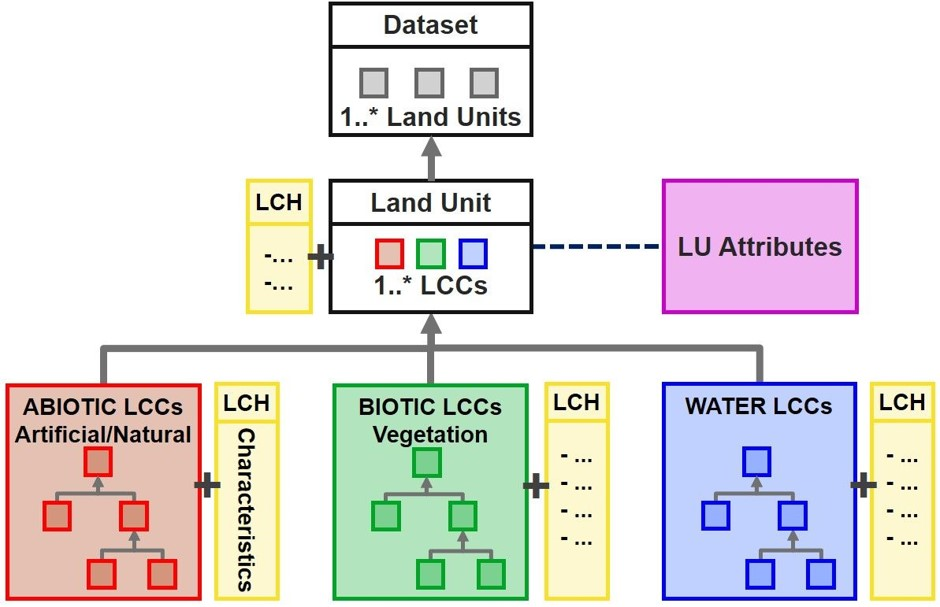
\includegraphics[width=0.75\textwidth]{figs_01/eagle_structure.png}
            \caption{Caption}
            \label{fig:eagle_structure}
        \end{figure}

        \begin{figure}[H]
        \centering
        \begin{subfigure}[b]{0.48\textwidth}
            \centering
            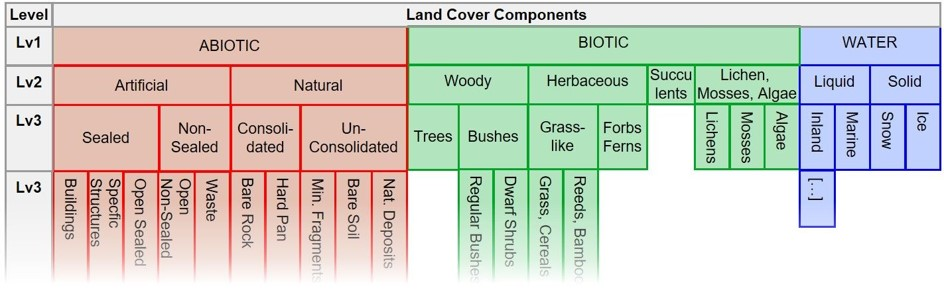
\includegraphics[width=\linewidth]{figs_01/eagle_landcover.png}
            \caption{Land Cover Components}
            \label{fig:eagle_landcover}
        \end{subfigure}
        \vspace{1em}
        \begin{subfigure}[b]{0.48\textwidth}
            \centering
            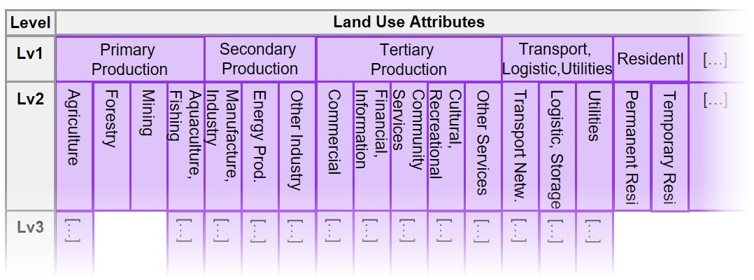
\includegraphics[width=\linewidth]{figs_01/eagle_landuse.png}
            \caption{Land Use Attributes}
            \label{fig:eagle_landuse}
        \end{subfigure}
        \vspace{1em}
        \begin{subfigure}[b]{0.48\textwidth}
            \centering
            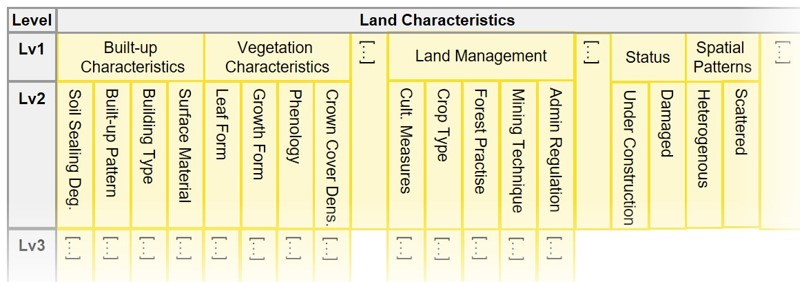
\includegraphics[width=\linewidth]{figs_01/eagle_landcharacteristics.png}
            \caption{Land Characteristics}
            \label{fig:eagle_landcharacteristics}
        \end{subfigure}
        
        \caption{A simplified(!) representation of the EAGLE concept and how it can be used to divide land units into categories based on hierarchical combinations of land cover, land use, and water presence. Source: \url{https://land.copernicus.eu/en/eagle}}
        \label{fig:eagle} % This should be inside the figure environment but outside any subfigure
        \end{figure}


        
        The framework should be expanded to incorporate reliable prediction uncertainty to make any produced maps more useful to researchers and decision-makers. Our first attempt was the model deviance from Chapter\@~\ref{cha:chapter3}, and is calculated by taking the standard deviation of predicted probabilities by each learner in an ensemble. While we found no relationship to the chance that a given prediction is correct, it turned out to be a relatively useful proxy for indicating the distance from the nearest training point of a given class in the feature space. In chapter 5, we compare three metrics that can have be used as proxies for error estimation: Highest predicted probability \citep{niculescu2005predicting}, margin of victory \citep{calderon2021high}, and IMP classification iteration. Predictions can be grouped based on these metrics, after which these groups can separately validated with calibration points to give a more fine-grained accuracy assessment. Comparing their performance to conformal prediction \citep{angelopoulos2023predictionpowered}, which promises statistical guarantees of correct error estimation, is a logical next step. Recently, the land cover community has begun adopting this technique for uncertainty estimation of land cover classification \citep{valle2023quantifying, singh2024uncertainty}.

        \subsubsection{Training Data Montage}

        Using a legend with an EAGLE-compliant hierarchy will allow us to more easily combine existing training datasets. This is usually very difficult due to different legends. For example, bigearthnet \citep{sumbul2021bigearthnet}. 

        An ideal improvement here would be to develop a multi-label classification system that can predict multiple levels of multiple hierarchies simultaneously. Summing the probabilities for combinations that are compatible and lead to a useful and interpretable class (such as two land cover labels \textit{herbaceous vegetation}, \textit{grass} and two land use labels 'primary production', 'grazing' to represent 'pasture')

        time-first space second approach might work well, especially for crops \citep{xu2021towards}

        hierarchical multilabel classification https://paperswithcode.com/task/hierarchical-multi-label-classification
        
        
        The ability of IMP to correct the bias of a model post-hoc also means that models don't need to be trained on datasets that respect class balance, like other mapping \citep{waldner2016towards,kleinewillinghofer2022unbiased}, as long as accurate area estimates are available. This means it can be combined with automated training data generation techniques that don't respect class distributions, such as extracting points from polygons \textit{en masse}, as was done in this thesis. It also means that training datasets with different distributions and classes can be combined if they are thematically compatible.

        It would be great if area estimates were available for all LUCAS land cover and land use combinations. IMP can help validate them!

        \citep{sumbul2021bigearthnet}

        \subsubsection{Featuring: Space}
        
        We primarily used a temporally aggregated version of the long-running Landsat archives due to its objective to make consistent time-series of maps and to enable the use of training data from legacy datasets such as CORINE. While the Landsat archives provide a consistent dataset spanning decades, its relatively low spatial, spectral, and temporal resolution limited the classification accuracy of several classes. 
        
        For example, different vegetation types are often best distinguished based on their profile in the electromagnetic spectrum \citep{xu2021towards,CITE, CITE}. Furthermore, crop types, in particular, benefit from high temporal resolution \citep{esch2014differentiation,xu2021towards}. Their growth cycles, during which their appearance and spectral profile changes drastically, combined with temporal dynamics such as crop rotation, fallow periods, and other practices, require a high frequency of EO data. Making use of Sentinel-2 imagery, with its revisit time of 10 days and higher spatial resolution (10~m), would have limited the time range of the maps to 2015 but might improve performance, as suggested in Chapter\@~\ref{cha:chapter2}. If the emphasis is on mapping longer time series, the framework could be significantly improved by incorporating the NASA Harmonized Landsat and Sentinel-2 (HLS), which combines the longevity of the Landsat program with the high temporal resolution of the Sentinel program \citep{claverie2018harmonized}.
        
        In the longer term, Landsat Next, scheduled to start providing data in 2030, promises substantial improvements while ensuring compatibility with both its own predecessors and other systems. The 26 spectral bands of this new iteration will match the 11 'heritage' bands of previous Landsat programs but will also contain 5 bands with similar spatial and spectral characteristics as Sentinel-2, improving revisit time from 16 to 6 days \citep{landsatnext2023}. Similarly, ESA's Copernicus Hyperspectral Imaging Mission for the Environment (CHIME) will have over 200 spectral bands and a revisit time of 12.5 days, revolutionizing hyperspectral earth observation \citep{nieke2023copernicus}. Meanwhile, the German Aerospace Center's recently launched Environmental Mapping and Analysis Program (EnMAP) system, with 228 hyperspectral bands and a revisit time of only 4 days, is particularly suitable for distinguishing vegetation types such as crops and tree species. It is already available and being used to map LULC, showcasing the utility of high spectral and temporal resolution in current remote sensing applications \citep{storch2023enmap, lekka2024appraisal}.

        % The recent advances and open availability of the Landsat and Sentinel programs, combined with the seemingly exponential increases in machine learning and high-performance computing, have dramatically enhanced the scale, quality, and quantity of work and research in the remote sensing field \citep{wulder2022fifty, claverie2018harmonized}.
    
        % Considering this, emerging and upcoming satellite programs with open data access can be used to improve the accuracy of frameworks and maps such as the ones presented in this thesis.

        When combined with training data that properly represents mapping 

        \subsubsection{One model to find them all, and in data bind them}

        \citep{xu2021towards} % An assessment of the input feature importance demonstrates that the AtLSTM, Transformer, and RF models all consider the period from weeks 11 to 20 (earlyJuly to late-August) as a key growth period and the shortwave infrared band as the critical band for corn and soybean discrimination. Hidden feature analysis suggests that the AtLSTM model accumulates the useful information over the growth period, while the Transformer model extracts the temporal dependencies that contribute important information to high-level feature learning. The learned features contain more effective and refined information than the raw input features and thus are better suited for crop classification

                The ideal model to classify this would be a multi-labeling classifier. Multi-labeling classifiers can predict several overlapping categories and have been used in [EXAMPLES]

        hierarchical multi-label classification!
        
    \subsection{Mapping everywhere: Moving beyond Europe}

        The framework presented in this thesis relies on openly available land cover samples for training and validation, and benefits greatly from accurate area estimates. Thanks to the efforts of European institutions such as the EEA and JRC, such things exists for Europe. Other continents, however, are not similarly fortunate. For example, the LUCAS land cover observations \citep{dandrimont2020harmonised} have allowed many global maps to be validated and compared in Europe \citep{gao2020consistency,venter2022global}, but this is more difficult to do in a standardized way in countries and continents that have a less detailed, reliable, or otherwise representative validation dataset.
        
        For that to work, we need global samples, global statistics, and take into account global differences.
        
        \subsubsection{Global data}
        
        datasets
        worldcereal \citep{boogaard2023worldcereal}

        worldcereal global temporary cropland extent \citep{lesiv2023global} %https://pure.iiasa.ac.at/id/eprint/18987/?template=default_internal
        cropharvest
        NASA cropharvest \citep{tseng2021cropharvest} % https://openreview.net/forum?id=JtjzUXPEaCu
        IMP-related: Global crop distribution maps from census to grid \citep{you2014generating}
        mapping global cropping system: challenges, opportunties, and future perspectives \citep{you2022mapping}

        \subsubsection{Global statistics}

        IMP quantifies model bias in the cut-off probability values for each class and iteration to make sure the bias is countered in the final hard-class classification. This might be generalizable to areas where you don't have area estimates if the confusion between classes is similar. You could store the probability threshold for each class at each iteration and apply them to probabilities predicted by the same model for a different area. This can be explored by mapping neighboring NUTS2 areas of the ones we have already mapped, using the cutoff values of their originally mapped neighbor. We can then 'pixel count', and compare the counts to the area estimates. This could make the method applicable for areas that are less meticulously quantified than Europe. This will still require area estimations to be done in some representative locations, but does not require continent- or country-wide surveys.
        
        \subsubsection{Global differences}

        Different regions have different classes and different ways of keeping track of them. This is caused by differences in administrative norms and capacity, but also due to different contexts and needs.

        % Expand on how different countries and continents have different norms and capacities, contexts and needs
        different biomes = different classes, different crops, classes look different
        
        different growing seasons = different time scales. In europe, crops need to be distinguished in july \citep{esch2014differentiation,xu2021towards} but this is very different in the tropics, where crops may grow all year round [???, CITE]
        
        % How do we deal with this?
        This can be solved in different ways: Train one model to recognize them all. If it works well, it will simply not map them in regions where they don't exist. This may not be feasible yet. You can also make different maps of different regions that are tailored to them by means of which classes, temporal extent and resolution. For example, WorldCereal global maps are comprised of a collection of regional maps, each characterized by its own definition of agricultural seasons \citep{tricht2023worldcereal}

    \subsection{Mapping all the time: Temporal resolution and range}

        Importance of temporal resolution

        Challenges in time-series analysis

        Technological advancements

        Applications of time-series analysis

        Future directions

        Monitoring RAD
    
        Time series analysis bfast avocado
    
        \citep{masolele2024mapping}
    
        It is important to validate annual large-scale maps with up-to date validation data to ensure there is no dataset drift and to properly quantify accuracy and uncertainty \citep{tsendbazar2021towards}
    

        
        

      
    
    
    
    % \subsection{Reflection: do we really need these maps? What kind of maps do we really need?}

    %     maps without users are meaningless
    %     wrong maps with users are dangerous \citep{bastin2019global}
    %     good maps with the wrong users are even more dangerous: 
    % Poachers \citep{beery2021can}- 
    % soil carbon, food and beverage companies are looking to reduce their carbon footprint  want to keep polluting. Disaster analysis maps are used by investors and insurance companies, buying land. Poachers etc. Do farmers benefit from cropland maps? No.
    % Exponential benefit to those who are already rich and powerful.
    
    % Spatial resolution:
        
    % temporal resolution:
    % crop mapping annually is difficult: you need sub-annual maps to do it properly. But where does this end? Daily maps? Multiple satellites flying in 
    
%     \subsection{Reflection: Open Data}
%     mention cool suppliers of open data:
% Major TOM \citep{francis2024major}
%     https://radiant.earth/blog/2023/05/we-dont-talk-about-open-data/ (the case against open data: helping poachers etc.)
%     \subsection{Future maps}
    
%         

%         

%         Mention EAGLE legend

        
%         
    
    
            
                
            



        

